% !TEX root = main.tex

\section{Combinational Circuits}
\subsection{Boolean Expression Trees}
A ``combinational'' circuit is one in which the output is entirely determined by the inputs---it is a pure function, with no dependence on state or time (apart from the initial time it takes the circuit to compute the output; see below). As such, its behavior is completely determined by a truth table; as we have seen, this means that it corresponds to a logical expression built up from the inputs and our basic operators.

When implementing a Boolean expression as a digital circuit, it is conventional to use a two-dimensional graphical representation of the circuit. This is partly because the circuit will eventually be laid out on a physical circuit board or semiconductor chip, and the relative locations of the gates and their interconnections will be important (although we will not go to this level of detail), but also because it can be easier to examine some of the properties and behavior of a circuit in a graphical form.

One way to get such a graphical representation is simply to use the expression tree. For example, we may picture the expression $s=(a+b)\overline{ab}$ as in Figure~\ref{fig:exprtree}.
\begin{figure}
\[ \setlength{\unitlength}{0.75pt}
\begin{picture}(120,140)
\put(10,40){\makebox(0,0){$a$}}
\put(50,40){\makebox(0,0){$b$}}
\put(30,70){\makebox(0,0){\textsc{or}}}
\put(10,45){\line(1,1){20}}
\put(50,45){\line(-1,1){20}}
\put(70,10){\makebox(0,0){$a$}}
\put(110,10){\makebox(0,0){$b$}}
\put(90,40){\makebox(0,0){\textsc{and}}}
\put(70,15){\line(1,1){20}}
\put(110,15){\line(-1,1){20}}
\put(90,70){\makebox(0,0){\textsc{not}}}
\put(90,45){\line(0,1){20}}
\put(60,100){\makebox(0,0){\textsc{and}}}
\put(30,75){\line(3,2){30}}
\put(90,75){\line(-3,2){30}}
\put(60,130){\makebox(0,0){$s$}}
\put(60,105){\line(0,1){20}}
\end{picture} \]
\caption{Expression tree for $s=(a+b)\overline{ab}$}
\label{fig:exprtree}
\end{figure}

Of course, we are usually interested in circuits that may have multiple outputs, so we may use a forest of expression trees. Figure~\ref{fig:exprforest} shows a forest for the same expression as above, along with the additional output $c$ given by $ab$.
\begin{figure}
\[ \setlength{\unitlength}{0.75pt}
\begin{picture}(200,140)
\put(10,40){\makebox(0,0){$a$}}
\put(50,40){\makebox(0,0){$b$}}
\put(30,70){\makebox(0,0){\textsc{or}}}
\put(10,45){\line(1,1){20}}
\put(50,45){\line(-1,1){20}}
\put(70,10){\makebox(0,0){$a$}}
\put(110,10){\makebox(0,0){$b$}}
\put(90,40){\makebox(0,0){\textsc{and}}}
\put(70,15){\line(1,1){20}}
\put(110,15){\line(-1,1){20}}
\put(90,70){\makebox(0,0){\textsc{not}}}
\put(90,45){\line(0,1){20}}
\put(60,100){\makebox(0,0){\textsc{and}}}
\put(30,75){\line(3,2){30}}
\put(90,75){\line(-3,2){30}}
\put(60,130){\makebox(0,0){$s$}}
\put(60,105){\line(0,1){20}}
\put(150,70){\makebox(0,0){$a$}}
\put(190,70){\makebox(0,0){$b$}}
\put(170,100){\makebox(0,0){\textsc{and}}}
\put(150,75){\line(1,1){20}}
\put(190,75){\line(-1,1){20}}
\put(170,130){\makebox(0,0){$c$}}
\put(170,105){\line(0,1){20}}
\end{picture} \]
\caption{Expression forest for $s=(a+b)\overline{ab}$ and $c=ab$}
\label{fig:exprforest}
\end{figure}

Upon doing this, we might notice that the subtree for $ab$ is duplicated. It would be nice to share common parts of the circuit, thus giving us an expression DAG (directed acyclic graph) instead of a tree or forest. One way to do this is shown in Figure~\ref{fig:exprdag1}.
\begin{figure}
\[ \setlength{\unitlength}{0.75pt}
\begin{picture}(150,140)
\put(10,40){\makebox(0,0){$a$}}
\put(50,40){\makebox(0,0){$b$}}
\put(30,70){\makebox(0,0){\textsc{or}}}
\put(10,45){\line(1,1){20}}
\put(50,45){\line(-1,1){20}}
\put(100,10){\makebox(0,0){$a$}}
\put(140,10){\makebox(0,0){$b$}}
\put(120,40){\makebox(0,0){\textsc{and}}}
\put(100,15){\line(1,1){20}}
\put(140,15){\line(-1,1){20}}
\put(90,70){\makebox(0,0){\textsc{not}}}
\put(120,45){\line(-3,2){30}}
\put(60,100){\makebox(0,0){\textsc{and}}}
\put(30,75){\line(3,2){30}}
\put(90,75){\line(-3,2){30}}
\put(60,130){\makebox(0,0){$s$}}
\put(60,105){\line(0,1){20}}
\put(120,130){\makebox(0,0){$c$}}
\put(120,45){\line(0,1){80}}
\end{picture} \]
\caption{Expression DAG for $s=(a+b)\overline{ab}$ and $c=ab$}
\label{fig:exprdag1}
\end{figure}

We could also share the inputs rather than repeating them, as shown in Figure~\ref{fig:exprdag2}; this is still a DAG.
\begin{figure}
\[ \setlength{\unitlength}{0.75pt}
\begin{picture}(110,140)
\put(10,0){\makebox(0,0){$a$}}
\put(100,0){\makebox(0,0){$b$}}
\put(10,70){\makebox(0,0){\textsc{or}}}
\put(10,5){\line(0,1){60}}
\put(100,5){\line(-3,2){90}}
\put(100,40){\makebox(0,0){\textsc{and}}}
\put(10,5){\line(3,1){90}}
\put(100,5){\line(0,1){30}}
\put(70,70){\makebox(0,0){\textsc{not}}}
\put(100,45){\line(-3,2){30}}
\put(40,100){\makebox(0,0){\textsc{and}}}
\put(10,75){\line(3,2){30}}
\put(70,75){\line(-3,2){30}}
\put(40,130){\makebox(0,0){$s$}}
\put(40,105){\line(0,1){20}}
\put(100,130){\makebox(0,0){$c$}}
\put(100,45){\line(0,1){80}}
\end{picture} \]
\caption{Expression DAG for $s=(a+b)\overline{ab}$ and $c=ab$, with shared inputs}
\label{fig:exprdag2}
\end{figure}

Finally, instead of using the words \textsc{and}, \textsc{or}, and \textsc{not}, the convention is to use the following symbols; we also draw the DAG ``on its side,'' so that the flow from inputs to outputs is left-to-right:
\begin{center}
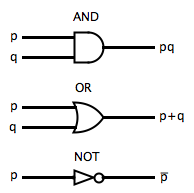
\includegraphics[width=\linewidth,height=!,scale=0.75]{graphics/AndOrNot.png}
%\begin{tikzpicture}[circuit logic US]
%\matrix[column sep=1cm]
%{
%  \node (a0) {$p$}; & \node {\textsc{and}}; & & \\
%  & \node [and gate] (a2) {}; & \node (a3) {$pq$}; & \\
%  \node (a1) {$q$}; & & & \\
%  \node (o0) {$p$}; & \node {\textsc{or}}; & & \\
%  & \node [or gate] (o2) {}; & \node (o3) {$p+q$}; & \\
%  \node (o1) {$q$}; & & & \\
%  & \node {\textsc{not}}; & \\
%  \node (n0) {$p$}; & \node [not gate] (n1) {}; & \node (n2) {$\overline{p}$}; \\
%};
%\draw (a2.input 1) -- ++(left:4mm) |- (a0.east);
%\draw (a2.input 2) -- ++(left:4mm) |- (a1.east);
%\draw (a2.output) -- (a3.west);
%\draw (o2.input 1) -- ++(left:4mm) |- (o0.east);
%\draw (o2.input 2) -- ++(left:4mm) |- (o1.east);
%\draw (o2.output) -- (o3.west);
%\draw (n1.input) -- (n0.east);
%\draw (n1.output) -- (n2.west);
%\end{tikzpicture}
\end{center}

The final result is a circuit diagram such as Figure~\ref{fig:exprcircuit}.
\begin{figure}
\begin{center}
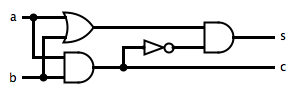
\includegraphics[width=!,height=!,scale=0.75]{graphics/HalfAdder.png}
%\begin{tikzpicture}[circuit logic US]
%\matrix[column sep=1cm]
%{
%  \node [or gate] (o1) {}; & & \node [and gate, yshift=-1mm] (a2) {}; & \node [yshift=-1mm] (s) {$s$}; \\
%  & \node [not gate] (n1) {}; & & \\
%  \node [and gate] (a1) {}; & & & \node (c) {$c$}; \\
%};
%\node (a) at ([xshift=-1.1cm]o1.input 1) {$a$};
%\node (b) at ([xshift=-1cm]a1.input 2) {$b$};
%\draw (a.east) -- (o1.input 1);
%\draw[*-] (b.east) ++(3mm,-0.8mm) |- (o1.input 2);
%\draw[*-] (a.east) ++(5mm,0.8mm) |- (a1.input 1);
%\draw (b.east) -- (a1.input 2);
%\draw (o1.output) -- ++(right:2cm) |- (a2.input 1);
%\draw (a2.output) -- (s.west);
%\draw (a1.output) -- (c.west);
%\draw[*-] (a1.output) ++(5mm,-0.8mm) |- (n1.input);
%\draw (n1.output) -- ++(right:0.5cm) |- (a2.input 2);
%\end{tikzpicture}
\end{center}
\caption{Circuit diagram for $s=(a+b)\overline{ab}$ and $c=ab$}
\label{fig:exprcircuit}
\end{figure}

It is important to realize, though, that this is just another presentation of the logical expressions we started with. Any set of Boolean expressions may be drawn this way, and any circuit where all of the information flows from left to right may be read as a set of expressions.

In addition to visualizing the layout of gates in a digital circuit, a circuit diagram may be used to ``trace'' its operation on particular inputs. For example, Figure~\ref{fig:exprcircuit11} is our example circuit annotated with \0/\1 logic values on each wire, to trace its behavior when both inputs $a$ and $b$ are 1. Since the logic values flow from left to right, the output of each successive gate may be determined from its inputs. By tracing each combination of inputs, we may construct a truth table corresponding to the circuit; the result is
\[ \begin{array}{cc|cc}
a  & b  & c & s\\ \hline
\0 & \0 & \0 & \0\\
\0 & \1 & \0 & \1\\
\1 & \0 & \0 & \1\\
\1 & \1 & \1 & \0
\end{array} \]
\begin{figure}
\begin{center}
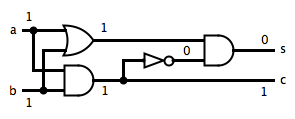
\includegraphics[width=!,height=!,scale=0.75]{graphics/HalfAdder11.png}
\end{center}
\caption{Annotated diagram for $s=(a+b)\overline{ab}$ and $c=ab$ when $a=1$ and $b=1$}
\label{fig:exprcircuit11}
\end{figure}

\paragraph{Implementation of Logic Gates}

It is useful to have some idea of how digital logic gates are built out of lower-level electronic devices such as transistors. For our purposes, a transistor is a voltage-controlled switch: when the voltage is high, the switch is closed (that is, it conducts electricity); when the voltage is low, the switch is open (breaking the connection). Figure~\ref{fig:nmosgates} shows n-type metal-oxide-semiconductor (NMOS) implementations of \textsc{not}, \textsc{nor}, and \textsc{nand} gates; we will study these instead of the more common complementary MOS (CMOS) gates, because they are slightly simpler---CMOS has the practical advantage of using significantly less power, at the cost of doubling the number of transistors, but the basic principles are very similar.

\begin{figure}
\begin{center}
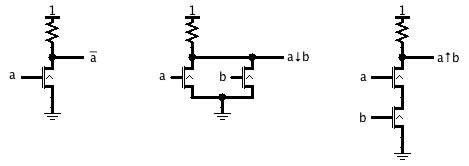
\includegraphics[width=!,height=!,scale=0.75]{graphics/NMOSgates.png}
\end{center}
\caption{NMOS implementations of \textsc{not}, \textsc{nor}, and \textsc{nand} gates}
\label{fig:nmosgates}
\end{figure}

The \textsc{not} gate consists of a single transistor in the lower half: the ``gate'' on the left is connected to the input signal, $a$; the ``source'' at the bottom is connected to ground, and the ``drain'' at the top is connected to the output, $\overline{a}$, and a ``pull-up'' resistor (the jagged line) whose other end is at the high voltage level. When $a=\0$ and the switch is open (so the transistor effectively has infinite resistance), the output will be pulled high (so $\overline{a}=\1$). When $a=\1$ and the switch is closed, the lower resistance through the transistor will pull the output low (so $\overline{a}=\0$).

The \textsc{nor} gate uses two transistors in parallel: if either $a$ or $b$ is high, then the output will be pulled low. Conversely, the \textsc{nand} gate uses two transistors in series: both have to be closed (so $a=b=\1$) for the output to be pulled to \0. Here are the conventional circuit symbols for \textsc{nand} and \textsc{nor} gates (note that the circle on the output indicates negation, just like on the \textsc{not} gate; the unnegated version of \textsc{not}, drawn as a simple triangle, is known as a ``buffer,'' because it copies its input to its output unchanged, after a short delay):
\begin{center}
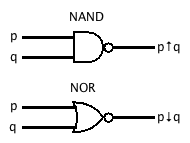
\includegraphics[width=!,height=!,scale=0.75]{graphics/NandNor.png}
\end{center}

Those three gates are the simplest to implement with transistors. As we saw in Section~\ref{ssec:OtherBooleanOps}, all other Boolean operators can be constructed from \textsc{nand} alone, or \textsc{nor} alone. For example, an \textsc{and} gate is a \textsc{nand} followed by a \textsc{not}, so it can be built out of three transistors; an \textsc{or} gate also takes three, using a \textsc{nor} and a \textsc{not}. In the next section, we will see another way to construct circuits using only \textsc{nand} gates.

\begin{tailquote}
Claude Shannon (1916--2001), known as ``the father of information theory,'' wrote his master's thesis at MIT in 1937. Entitled ``A Symbolic Analysis of Relay and Switching Circuits,'' it has been called the most influential master's thesis of the 20\textsuperscript{th} century. In it, he showed how to systematically turn expressions of Boolean algebra into circuits made up of switches.
\end{tailquote}
\begin{exercises}
\problem For each of the following Boolean expressions, draw a corresponding circuit diagram. Try to reuse as many common intermediate results as you can.
\begin{enumerate}
\item $x=\overline{(\overline{a}+b)}+\overline{\overline{b}}+\overline{a}$
\item $x=\overline{\overline{c}a}+\overline{b}$, $y=\overline{\overline{c}b}+\overline{a}$
\item $x=abc+abd+acd+bcd$
\end{enumerate}

\problem For each of the following truth tables, draw a corresponding circuit diagram. \textit{(Hint: First extract one or more Boolean expressions in DNF from the table.)}
\begin{enumerate}
\item \( \begin{array}[t]{cc|cc}
a  & b  & x  & y\\ \hline
\0 & \0 & \0 & \1\\
\0 & \1 & \1 & \0\\
\1 & \0 & \1 & \0\\
\1 & \1 & \0 & \1
\end{array} \)
\item \( \begin{array}[t]{ccc|c}
a  & b  & c  & x\\ \hline
\0 & \0 & \0 & \0\\
\0 & \0 & \1 & \0\\
\0 & \1 & \0 & \0\\
\0 & \1 & \1 & \1\\
\1 & \0 & \0 & \0\\
\1 & \0 & \1 & \1\\
\1 & \1 & \0 & \1\\
\1 & \1 & \1 & \1
\end{array} \)
\end{enumerate}

\problem For each of the following circuit diagrams, write the corresponding Boolean expressions, then trace the output on each combination of inputs and summarize the results in a truth table.
\begin{enumerate}
\item 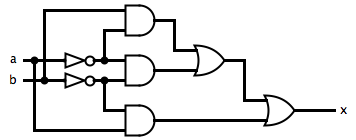
\includegraphics[width=!,height=!,scale=0.75]{graphics/Exercise5213a.png}
\item 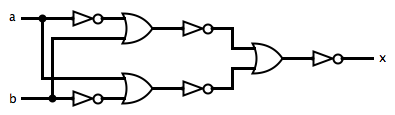
\includegraphics[width=!,height=!,scale=0.75]{graphics/Exercise5213b.png}
\end{enumerate}
\end{exercises}

\subsection{Circuit Simplification}\label{sec:circsimp}
As noted above, a physical circuit does have some dependence on time, since each device in the circuit requires a non-zero time to respond to a change in its inputs. A more precise model needs to take these delays into account---a circuit is modeled by a Boolean expression \emph{plus} a set of delay factors (other cost measures may also be important: power consumption, heat production, area occupied, \textit{etc.}, but we will focus on the delay issue here). We will make the simplifying assumption that all gates have the same delay time, so we will measure the total delay of a circuit in terms of the number of gate delays required before the output values accurately reflect a change to the input values.

Given a combinational circuit, we may compute the delay, also known as the \textit{span}, by finding the number of gates on the longest path (the ``critical path'') from an input to an output. For example, the circuit in Figure~\ref{fig:exprcircuit} has a span of three gate delays, with the critical path going from either $a$ or $b$ to $s$, passing through an \textsc{and}, a \textsc{not}, and another \textsc{and} gate. Note that this is a conservative estimate of the delay required, although for certain inputs the output may become stable sooner---for example, if $a$ and $b$ both change to \0, then after one gate delay the output of the \textsc{or} and the first \textsc{and} will both be \0; that means that in this case, output $c$ will be determined after one gate delay, while output $s$ will be determined after two gate delays (because as soon as one input to the second \textsc{and} is \0, its output will become \0 after one more gate delay regardless of the other input). However, other combinations of inputs may well take the entire three gate delays to correctly determine the value of $s$.

One approach to reducing the delay of a circuit is to use the disjunctive normal form, also known as the ``sum-of-products'' (see Section~\ref{ssec:DNF}). Since an expression in DNF is the \textsc{or} of a collection of terms which are the \textsc{and} of some number of literals, and a literal is either an input or a negated input, the corresponding circuit can be constructed in three layers:
\begin{center}
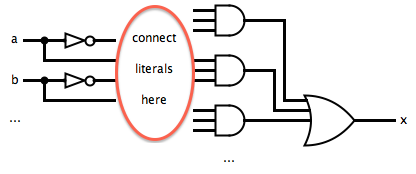
\includegraphics[width=!,height=!,scale=0.75]{graphics/DNFlayers.png}
\end{center}

An interesting property of the sum-of-products representation falls out of the De Morgan laws. Since $ab+cd=\overline{\overline{ab}\cdot\overline{cd}}=(a\uparrow b)\uparrow(c\uparrow d)$, the two layers of \textsc{and} and \textsc{or} gates may be replaced entirely with \textsc{nand} gates to get an equivalent circuit!
\begin{center}
\includegraphics[width=!,height=!,scale=0.75]{graphics/DNFlayersNand.png}
\end{center}

Unfortunately, this does not mean that any Boolean expression can be computed by a circuit with only three gate delays. One problem comes when we need \textsc{and} and \textsc{or} gates (or \textsc{nand} gates) with more than two inputs---in general, with $n$ input variables, there may be \textsc{and} gates that need $n$ literal inputs, and there could be on the order of $2^n$ gates in the \textsc{and} level, requiring an \textsc{or} gate with that many input lines. We will see in the next section how to build gates with a larger number of inputs out of gates with just two inputs.

Another problem with DNF comes if we use the full DNF expression extracted from a truth table. Recall the full DNF expression that we extracted from the truth table for $p\rightarrow q$ in Section~\ref{ssec:OtherBooleanOps}: $\overline{p}\cdot\overline{q}+\overline{p}q+pq$. We were able to use Boolean identities to find an equivalent DNF expression, $\overline{p}+q$ (which only needs two gate delays, since the \textsc{and} layer disappears). There are general techniques for finding simpler DNF expressions such as this; we will look at a simple technique called a \textit{Karnaugh map}, although for computer implementation the related Quine-McCluskey algorithm is better (and for large numbers of input variables a heuristic approach is necessary).

A Karnaugh map is a way of visualizing entries in a truth table so that adjacent entries only differ on the value of one input variable. For example, the entry for $\overline{p}q$ will be next to the entry for $pq$. If adjacent entries each contain 1, meaning that those terms would participate in the full DNF expression, then they may be replaced by a single term with just the variables that are the same: in the example, this corresponds to the simplification $\overline{p}q + pq=(\overline{p}+p)q=1q=q$.

For two input variables, a Karnaugh map is a $2\times 2$ array:
\[ \begin{array}{r|cc}
& \overline{q} & q\\ \hline
\overline{p} & x_{00} & x_{01}\\
p & x_{10} & x_{11}
\end{array} \]
This is just a compact rearrangement of the truth table:
\[ \begin{array}{cc|c}
p & q & x\\ \hline
\0 & \0 & x_{00}\\
\0 & \1 & x_{01}\\
\1 & \0 & x_{10}\\
\1 & \1 & x_{11}
\end{array} \]
However, note that the adjacent cell condition is true: horizontally adjacent cells only differ on $q$, while vertically adjacent cells only differ on $p$.

Once we have laid out the Karnaugh map, a simplified expression may be read off by finding a way to cover all of the 1's in the map with ``implicants.'' An implicant is a rectangle whose side lengths are a power of 2; it corresponds to finding a collection of adjacent cells in the map (all of which contain 1) that all agree on some of the input literals and that collectively include all combinations (negated or not) of the other input variables. The resulting term for an implicant is just the product of the common literals among all the cells covered by the implicant.

On a $2\times 2$ map, the only implicants are individual cells ($1\times 1$), a row ($1\times 2$), a column ($2\times 1$), or the entire map ($2\times 2$). The cells correspond to terms such as $p\overline{q}$, the rows are either $\overline{p}$ or $p$, the columns are either $\overline{q}$ or $q$, and the entire map is $1$ (the empty product). To get the simplest expression, we want to take the fewest number of the largest possible implicants that between them cover all of the 1's in the map. Implicants may overlap, as long as all of (and only) the 1's are covered by at least one implicant.

Here is the example again. First the truth table for $p\rightarrow q$:
\[ \begin{array}{cc|c}
p & q & x\\ \hline
\0 & \0 & \1\\
\0 & \1 & \1\\
\1 & \0 & \0\\
\1 & \1 & \1
\end{array} \]
As a Karnaugh map, this is:
\[ \begin{array}{r|cc}
& \overline{q} & q\\ \hline
\overline{p} & \1 & \1\\
p & \0 & \1
\end{array} \]
The best way to cover this map with implicants is to take the first row and the second column. That gives the simplified terms $\overline{p}$ and $q$, so the final simplified expression is $\overline{p} + q$. Here is the map with the implicants outlined:
\[ \begin{array}{r|cc}
& \overline{q} & q\\ \hline
\overline{p} & \tikzmark{left1}\1 & \tikzmark{left2}\1\tikzmark{right1}\\
p & \0 & \1\tikzmark{right2}
\end{array}
\DrawBox[blue]{left1}{right1}
\DrawBox[red]{left2}{right2} \]

A Karnaugh map can also work with three or four input variables, producing either a $2\times 4$ or a $4\times 4$ array. The same procedure applies, with three complications:
\begin{enumerate}
\item To satisfy the adjacent cell condition, successive rows or columns must change only one variable at a time: for example, the rows might be labelled in order $\overline{p}\cdot\overline{q}$, $\overline{p}q$, $pq$, and $p\overline{q}$;
\item Implicants may be 1, 2, or 4 rows tall by 1, 2, or 4 columns wide; and
\item Implicants may ``wrap around'' from one side of the map to the other.
\end{enumerate}
For example, on a $4\times 4$ map, one possible implicant is the middle two rows; another is the leftmost and rightmost columns (wrapping horizontally); a third is the $2\times 2$ block consisting of the middle two elements of the top row and the middle two elements of the bottom row (wrapping vertically); a final example is the last two elements of the third row. See Figure~\ref{fig:KarnaughImplicants} for these examples.

\begin{figure}
Middle two rows ($q$):
\[ \begin{array}{r|cccc}
& \overline{r}\cdot\overline{s} & \overline{r}s & rs & r\overline{s}\\ \hline
\overline{p}\cdot\overline{q} & & & & \\
\overline{p}q & \tikzmark{left1}1 & 1 & 1 & 1\\
pq & 1 & 1 & 1 & 1\tikzmark{right1}\\
p\overline{q} & & & &
\end{array}
\DrawBox[blue]{left1}{right1} \]

Leftmost and rightmost columns ($\overline{s}$):
\[ \begin{array}{r|cccc}
& \overline{r}\cdot\overline{s} & \overline{r}s & rs & r\overline{s}\\ \hline
\overline{p}\cdot\overline{q} & \tikzmark{left1}1 & & & \tikzmark{left2}1\\
\overline{p}q & 1 & & & 1\\
pq & 1 & & & 1\\
p\overline{q} & 1\tikzmark{right1} & & & 1\tikzmark{right2}
\end{array}
\DrawBoxW[blue]{left1}{right1}
\DrawBoxE[blue]{left2}{right2} \]

Middle elements of top and bottom rows ($\overline{q}s$):
\[ \begin{array}{r|cccc}
& \overline{r}\cdot\overline{s} & \overline{r}s & rs & r\overline{s}\\ \hline
\overline{p}\cdot\overline{q} & & \tikzmark{left1}1 & 1\tikzmark{right1} & \\
\overline{p}q & & & &\\
pq & & & &\\
p\overline{q} & & \tikzmark{left2}1 & 1\tikzmark{right2} &
\end{array}
\DrawBoxN[blue]{left1}{right1}
\DrawBoxS[blue]{left2}{right2} \]

Last two elements of the third row ($pqr$):
\[ \begin{array}{r|cccc}
& \overline{r}\cdot\overline{s} & \overline{r}s & rs & r\overline{s}\\ \hline
\overline{p}\cdot\overline{q} & & & & \\
\overline{p}q & & & &\\
pq & & & \tikzmark{left1}1 & 1\tikzmark{right1}\\
p\overline{q} & & & &
\end{array}
\DrawBox[blue]{left1}{right1} \]
\caption{Some examples of Karnaugh map implicants}
\label{fig:KarnaughImplicants}
\end{figure}

A Karnaugh map also allows us to find simple circuits in the case that some combinations of inputs will never occur, so that we do not care what the output is in those rows of the truth table. By entering a ``don't care'' value, such as X, in the map, we have the freedom to either ignore or include those cells when covering the map with implicants; by including a cell with an X along with a group of 1's, we might be able to construct a larger (and hence simpler) implicant.

For example, suppose we have the following truth table for a four-variable Boolean expression (this represents the inputs that are binary numbers less than ten and divisible by three):
\[ \begin{array}{cccc|c}
p & q & r & s & x\\ \hline
\0 & \0 & \0 & \0 & \1\\
\0 & \0 & \0 & \1 & \0\\
\0 & \0 & \1 & \0 & \0\\
\0 & \0 & \1 & \1 & \1\\
\0 & \1 & \0 & \0 & \0\\
\0 & \1 & \0 & \1 & \0\\
\0 & \1 & \1 & \0 & \1\\
\0 & \1 & \1 & \1 & \0\\
\1 & \0 & \0 & \0 & \0\\
\1 & \0 & \0 & \1 & \1\\
\1 & \0 & \1 & \0 & X\\
\1 & \0 & \1 & \1 & X\\
\1 & \1 & \0 & \0 & X\\
\1 & \1 & \0 & \1 & X\\
\1 & \1 & \1 & \0 & X\\
\1 & \1 & \1 & \1 & X
\end{array} \]
As a Karnaugh map, this is:
\[ \begin{array}{r|cccc}
& \overline{r}\cdot\overline{s} & \overline{r}s & rs & r\overline{s}\\ \hline
\overline{p}\cdot\overline{q} & \1 & \0 & \1 & \0\\
\overline{p}q & \0 & \0 & \0 & \1\\
pq & X & X & X & X\\
p\overline{q} & \0 & \1 & X & X
\end{array} \]
The \1's, plus some of the X's, may be covered by four implicants: $\overline{p}\cdot\overline{q}\cdot\overline{r}\cdot\overline{s}$, $\overline{q}rs$, $qr\overline{s}$, and $ps$. Note that the second implicant wraps around from the third cell on the top row to the third cell (with an X, which is also covered by the $ps$ implicant) on the bottom row; if it were just the \1 on the top row, then the term would be $\overline{p}\cdot\overline{q}rs$, which is not as simple. Here are the cells that end up being covered:
\[ \begin{array}{r|cccc}
& \overline{r}\cdot\overline{s} & \overline{r}s & rs & r\overline{s}\\ \hline
\overline{p}\cdot\overline{q} & \tikzmark{left1}\1\tikzmark{right1} & \0 & \tikzmark{left2a}\1\tikzmark{right2a} & \0\\
\overline{p}q & \0 & \0 & \0 & \tikzmark{left3}\1\\
pq & X & \tikzmark{left4}X & X & X\tikzmark{right3}\\
p\overline{q} & \0 & \1 & \tikzmark{left2b}X\tikzmark{right2b}\tikzmark{right4} & X
\end{array}
\DrawBox[blue]{left1}{right1}
\DrawBoxN[red,rounded corners=3pt]{left2a}{right2a}
\DrawBoxS[red,rounded corners=3pt]{left2b}{right2b}
\DrawBox[green]{left3}{right3}
\DrawBox[purple]{left4}{right4} \]
Therefore, the simplified expression is $\overline{p}\cdot\overline{q}\cdot\overline{r}\cdot\overline{s} + \overline{q}rs + qr\overline{s} + ps$. This may be computed by the following circuit:
\begin{center}
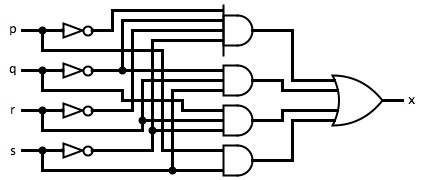
\includegraphics[width=!,height=!,scale=0.75]{graphics/KarnaughExample.png}
\end{center}
In the next section, we will see how to implement this with a total delay of 5, using only two-input \textsc{and} and \textsc{or} gates.

The final difficulty with building low-delay circuits from DNF expressions is that, even with the simplification provided by something like a Karnaugh map, many Boolean functions lead to an exponential blowup when expressed in DNF. In the worst case, an expression with $n$ input variables may require $O(2^n)$ terms in a sum-of-product representation---consider the case of a Karnaugh map where the \1's are in a checkerboard arrangement, so that none are adjacent. When $n$ is large enough, it might not even be practical to consider the truth table at all; for example, a circuit that can add two 32-bit numbers requires 64 input lines, which would lead to a truth table with $2^{64}\approx 10^{19}$ entries. The next section will also discuss approaches to this kind of problem.

\begin{tailquote}
Maurice Karnaugh [pronounced ``CAR-no''] (1924--) developed his map method in 1953, based on a 1952 paper by Edward Veitch (1924--2013), ``A Chart Method for Simplifying Truth Functions.'' The major difference between Karnaugh's and Veitch's diagrams was the ordering of the columns and rows---Veitch put them in straight binary order, while Karnaugh rearranged them to make adjacent cells differ by only one variable. Veitch's approach makes sense if you picture the diagram as showing layers of a cube or hypercube, and arguably extends more readily to five or six variables, but Karnaugh's approach became more popular.
\end{tailquote}

\begin{exercises}
\problem For each of the following Boolean expressions, compute the total delay of the direct translation of the expression into a circuit.
\begin{enumerate}
\item $\overline{(\overline{p}+q)}+(\overline{\overline{q}}+\overline{p})$
\item $(\overline{\overline{r}p}+\overline{q})(\overline{\overline{r}q}+\overline{p})$
\item $(((p+q)(q+r))\,(r+s))\,(((p+r)(q+s))\,(p+s))$
\end{enumerate}

\problem For each of the expressions in the previous problem, use a Karnaugh map to find an equivalent sum-of-products expression, and draw the resulting circuit.

\problem Suppose we want to build a counter that cycles through the numbers 0, 1, 2, 3, 4, and back to 0. One element of this counter will be a circuit that takes the current number, expressed in binary, and outputs the next number. Here is the truth table for this function, with three inputs ($a$, $b$, and $c$) and three outputs ($x$, $y$, and $z$):
\[ \begin{array}{ccc|ccc}
a & b & c & x & y & z\\ \hline
\0 & \0 & \0 & \0 & \0 & \1\\
\0 & \0 & \1 & \0 & \1 & \0\\
\0 & \1 & \0 & \0 & \1 & \1\\
\0 & \1 & \1 & \1 & \0 & \0\\
\1 & \0 & \0 & \0 & \0 & \0\\
\1 & \0 & \1 & X & X & X\\
\1 & \1 & \0 & X & X & X\\
\1 & \1 & \1 & X & X & X\\
\end{array} \]
Since the counter should never reach numbers 5, 6, or 7, we do not care about the output when $abc$ is \1\0\1, \1\1\0, or \1\1\1. Use Karnaugh maps to find a simple circuit for this function.

\problem\label{ex:BCD} In binary-coded decimal (BCD), four bits are used to represent the numbers 0 (\0\0\0\0) through 9 (\1\0\0\1); the other six bit patterns (\1\0\1\0 through \1\1\1\1) are unused. BCD is often used in circuits where decimal numbers need to be displayed; a common device for doing so is the ``seven-segment display.'' Using only seven elements (for example, light-emitting diodes), we may form a reasonable approximation of all the digits 0--9: \textifsym{0123456789}. Construct a truth table with four inputs and seven outputs showing how to produce these characters from input in BCD (be sure to include a diagram indicating which output column corresponds to which display element). Use Karnaugh maps to design a relatively simple circuit that implements a seven-segment decoder.

\problem Exercise~\ref{ex:CNF} of Section~\ref{ssec:DNF} examines conjunctive normal form (CNF), the dual of DNF. Explore what kind of circuits result from CNF, and how to extract a simplified CNF expression from a Karnaugh map \textit{(Hint: look at blocks of \0's.)}.
\end{exercises}

\subsection{Common Circuit Components}
Just as a complicated piece of software is never written from scratch entirely from the most basic program statements, a complicated hardware design is not approached purely at the gate level. Where a programmer will break the task into a hierarchy of objects and functions, relying on familiar idioms and existing code from program libraries to avoid reinventing the wheel, a hardware designer will use a hierarchy of functional blocks, relying on familiar patterns and existing libraries of subcircuits.

We have already seen one of these common components---the sample circuit in Figure~\ref{fig:exprcircuit} is known as the ``half adder.'' If $a$ and $b$ represent one-bit binary numbers, then $s$ is their one-bit sum and $c$ is the carry into the next bit. For example, when $a$ and $b$ are both \1, $s$ is \0 and $c$ is \1; in binary, this says $1+1=10$. We may represent this block in a circuit diagram with an appropriately named box:
\begin{center}
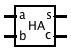
\includegraphics[width=!,height=!,scale=0.75]{graphics/HalfAdderSymbol.png}
\end{center}
It is called a half adder because, when you are adding multiple columns of bits, it only does half the work: it adds the two bits for a column, but it doesn't add in the carry from the next smaller column. A ``full adder'' takes three inputs: $a$ and $b$, plus the incoming carry, $c_\textit{\scriptsize in}$. The outputs are $s$, the sum that stays in the column, plus the outgoing carry to the next column, $c_\textit{\scriptsize out}$. We may build a full adder out of two half adders by first adding $a$ to $b$, then adding $c_\textit{\scriptsize in}$; since the highest total in a full adder is three (\1\1), we will never have a carry out of more than one of the half adders, so the resulting $c_\textit{\scriptsize out}$ is just the \textsc{or} of the two half adder carries. Here is the circuit with its block symbol and its truth table:
\[
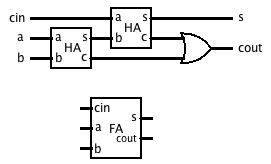
\includegraphics[width=!,height=!,scale=0.75]{graphics/FullAdder.png}\hspace{1cm}
\begin{array}[b]{ccl|rc}
a & b & c_\textit{\scriptsize in} & c_\textit{\scriptsize out} & s\\ \hline
\0 & \0 & \0 & \0 & \0\\
\0 & \0 & \1 & \0 & \1\\
\0 & \1 & \0 & \0 & \1\\
\0 & \1 & \1 & \1 & \0\\
\1 & \0 & \0 & \0 & \1\\
\1 & \0 & \1 & \1 & \0\\
\1 & \1 & \0 & \1 & \0\\
\1 & \1 & \1 & \1 & \1
\end{array}
\]

Given a full adder, we may construct multiple-bit adders by ``cascading'' them, with the carry from each column feeding into the next. Here, for example, is a four-bit adder; the inputs are $a_3a_2a_1a_0$ and $b_3b_2b_1b_0$, plus an incoming carry $c_\textit{\scriptsize in}$ to column 0 (the one's column), and the outputs are $s_3s_2s_1s_0$, plus a carry from column 3 (the eight's column), $c_\textit{\scriptsize out}$:
\begin{center}
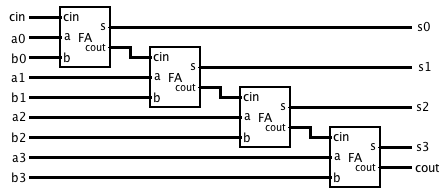
\includegraphics[width=!,height=!,scale=0.75]{graphics/4BitAdder.png}
\end{center}
Exercise~\ref{ex:cascade} explores whether this is a good design.

A common pattern in logic circuits is to use the \textsc{and} gate to ``enable'' (or disable) some signal. For example, in the half adder, the sum output, $s$, is true when one of the inputs is true ($a+b$), except it is disabled when there is a carry (both are true, $a\cdot b$). For another example, suppose we have a circuit which is supposed to compute one of two functions, either $f$ or $g$, depending on a ``select'' input; the circuit might look like this:
\begin{center}
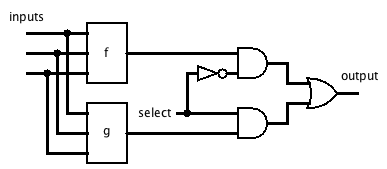
\includegraphics[width=!,height=!,scale=0.75]{graphics/ForG.png}
\end{center}
When \textit{select} is \0, the output is computed by $f$; when it is \1, the output is computed by $g$.

The idea of selecting from two signals may be generalized to using a $k$-bit input to select from one of up to $2^k$ signals; the result is known as a ``multiplexer'' (often abbreviated MUX). For example, with two select lines, $s_1s_0$, you can choose one of four inputs: $a_{00}$, $a_{01}$, $a_{10}$, or $a_{11}$. Each input is enabled by an appropriate combination of the select lines and their complements, then all four possibilities (of which at most one may be true) are combined with \textsc{or}. Here is the circuit and its common symbol:
\begin{center}
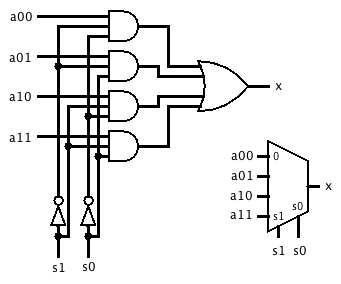
\includegraphics[width=!,height=!,scale=0.75]{graphics/MUX.png}
\end{center}

Note the similarity of the multiplexer circuit to the layers of the sum-of-products circuit from Section~\ref{sec:circsimp}. If we view the input lines $a_{ij}$ as the enabling inputs, then a multiplexer gives a direct way of implementing a truth table: hard-wire the input lines to \0 or \1 according to the corresponding entries in the truth table, then use the select lines to choose the desired row to send to the output. For example, if $a_{01}$ and $a_{10}$ are both tied to \1, while $a_{00}$ and $a_{11}$ are \0, then the output of the multiplexer will be the exclusive-\textsc{or} of $s_1$ and $s_0$.

The opposite of a multiplexer is a ``demultiplexer'' (DEMUX). It takes one input signal plus $k$ select lines, and delivers the input signal to one of $2^k$ output lines. A special case is known as a ``($k$-bit) decoder'': if the input signal is fixed at \1, then the decoder will send a \1 to exactly one of its output lines. Alternately, a demultiplexer can be viewed as a decoder with an ``enable'' input, where the selected output line will be \1 only if the enabling input signal is \1. Here is the common symbol for a four-line demultiplexer:
\begin{center}
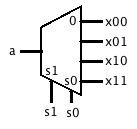
\includegraphics[width=!,height=!,scale=0.75]{graphics/DEMUX.png}
\end{center}
The implementation of this circuit is left as an exercise.

\begin{tailquote}
Edward F.~Moore (1925--2003) described his finite state machine model (see Section~\ref{sec:moore}) in a 1956 paper entitled ``Gedanken-Experiments on Sequential Machines.'' In it, he considered machines as ``black boxes,'' completely determined by their inputs and outputs (as an extreme, he considered ``infernal machines,'' where one possible output is that it explodes\ldots). The combinational circuits in this section are the special case of boxes where there is no state dependence on previous inputs.
\end{tailquote}
\begin{exercises}
\problem\label{ex:cascade} Compute the total gate delays for a half adder, a full adder, and a four-bit cascaded adder as described in this section. The total delay is the maximum number of gate delays between any input signal changing and all output signals stabilizing to reflect the changed input.

\problem Draw the circuit diagram for an implementation of a four-line demultiplexer.

\problem A ``parity bit generator'' is a circuit that takes some number of lines of input and produces one output which is \0 if an even number of the inputs are \1, and \1 if an odd number of the inputs are \1. If the input bits are transmitted along with the generated parity bit, then a recipient can check whether any single bit was mis-transmitted by ensuring that the total number of \1 bits received is even. A two-input parity bit generator is just the exclusive-\textsc{or} circuit, whose common symbol is:
\begin{center}
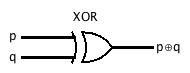
\includegraphics[width=!,height=!,scale=0.75]{graphics/XOR.png}
\end{center}
Give an implementation of a two-input parity bit generator using only \textsc{nand} gates, and then show how to use \textsc{xor} gates to build an eight-input parity bit generator.

\problem The opposite of a decoder is an ``encoder'': given $2^k$ input lines, the output will be a $k$-bit binary number representing which input is \1. In case more than one input line is \1, the output will give the highest such line number; this is known as a ``priority encoder.'' For example, when $k=3$, if lines $a_1$, $a_4$, and $a_5$ are all \1, while the rest are \0, then the output will be \1\0\1 (5 in binary). If no input line is \1, then the output will be \0\0\0. There is one additional output line, $g$ (the ``group'' signal) that will only be \1 if at least one of the inputs is \1; this allows us to tell the difference between no input and only line $a_0$ being \1.

Give a truth table for a four-input ($k=2$) priority encoder, then draw a circuit diagram that implements it.
\end{exercises}

\subsection{Divide-and-Conquer Design}
See Sections~13.5--7 of Aho \& Ullman.
\begin{exercises}
\problem Show how to construct a $2k$-input parity bit generator given a block that implements a $k$-input parity bit generator.

\problem Show how to construct a $2k$-input priority encoder given a block that implements a $k$-input priority encoder.
\end{exercises}


